\lstset{frame=tb,
	language=C++,
	aboveskip=3mm,
	belowskip=3mm,
	showstringspaces=false,
	columns=flexible,
	basicstyle={\small\ttfamily},
	numbers=none,
	numberstyle=\tiny,
	breaklines=true,
	breakatwhitespace=true,
	tabsize=3}

\chapter{Verificarea formală a problemei}

\section{Implementarea algoritmului}
    Implementarea algoritmului propriu-zis care rezolvă problema a fost primul și cel mai ușor pas.\par
    Am început prin crearea unei bucle care la fiecare pas alegea bancnota optimă, o adăuga în secvența de 
    bancnote considerată soluție și o scădea din sumă, fiind un algoritm tipic metodei Greedy.
    \begin{lstlisting}
    var rest:= sum;
    solution:= [0, 0, 0, 0, 0, 0];
    while (0 < rest)
        decreases rest 
        {
        index:= maxBanknote(rest);
        var banknote:= power(2, index);
        solution:= addValueToIndex(solution,1,index);
        rest:= rest - banknote;
    }
    \end{lstlisting}

    Acest algoritm era suficient pentru a rezolva problema, dar nu era suficient pentru a demonstra că soluția produsă este optimă.\par
    Considerăm o soluție optimă soluția de cost minim, costul fiind numărul de bancnote.
    
\section{Demonstrarea optimalității}
    \subsection{Schema verificării}
    \vspace{1cm}
    \begin{center}
        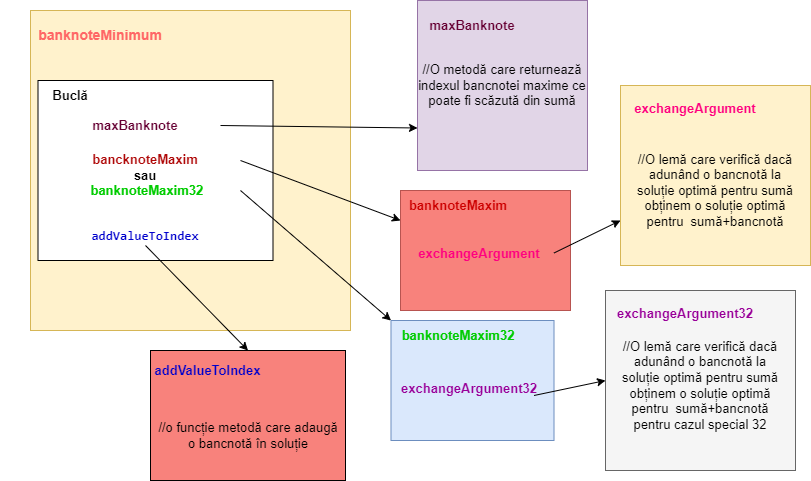
\includegraphics[width=1.0\textwidth]{verification_schema.png}\par
    \end{center}
    În schema de mai sus am exemplificat modul în care funcțiile, lemele și metodele se apelează una pe cealaltă pentru a demonstra faptul că soluția găsită este soluție optimă.\par

    \subsection{Condiții ca o soluția finală să fie optimă}
    $\bullet$ Pentru a avea o soluție optimă trebuie să avem o soluție validă (cu 6 elemente), care produce suma corectă
     și care are costul cel mai mic.\par
    $\bullet$ Pentru a avea o soluție optimă finală, pe parcursul construirii soluției, în buclă, trebuie menținută proprietatea
     de a alege soluția optimă locală pentru rest, iar suma soluțiilor optime locale să fie soluție optimă pentru sumă.\par
    $\bullet$ Soluția formată dintr-o bancnotă, cea aleasă în iterația curentă, produce o soluție optimă pentru suma 
    de valoare bancnotă, asigurând faptul că avem o soluție optimă locală.\par
    $\bullet$ O soluție optimă pentru suma $x$, adunată cu o soluție optimă pentru suma $y$ creează o soluție optimă pentru suma $x+y$, 
    asigurând faptul că suma soluțiilor locale creează soluția finală optimă.\par
    
\section{Pașii verificării}
    \subsection{banknoteMinimum}
    Am implementat algoritmul Greedy care rezolva Problema Bancnotelor cu bancnote puteri ale lui 2, 
    apoi am adăugat treptat condițiile care garantează că soluția găsită este soluție optimă.\par
    \begin{lstlisting}
    method banknoteMinimum(sum: int) returns(solution: seq < int > )
        requires sum >= 0
        ensures isValidSolution(solution)
        ensures isSolution(solution, sum)
        ensures isOptimalSolution(solution, sum) 
    {
        var rest:= sum;
        solution:= [0, 0, 0, 0, 0, 0];
        var index:= 0;
        assert isOptimalSolution(solution, sum - rest);
        while (0 < rest)
            invariant 0 <= rest <= sum
            invariant isValidSolution(solution)
            invariant addOptimRestEqualsOptimSum(rest, sum, solution)
            decreases rest 
        {
            index:= maxBanknote(rest);
            var banknote:= power(2, index);
            if (index != 5) 
            {
                banknoteMaxim(rest, sum, solution, index);
            } 
            else 
            {
                banknoteMaxim32(rest, sum, solution);
            }
            solution:= addValueToIndex(solution,1,index);
            rest:= rest - banknote;
        }
    }
    \end{lstlisting}
    \subsection{maxBanknote}
    Pentru a alege bancnota cea mai mare am creat funcția maxBanknote.\par
    \begin{lstlisting}
      method maxBanknote(sum: int) returns(index: int)
        requires sum > 0
        ensures 0 <= index <= 5
        ensures 0 <= power(2, index) <= sum
        ensures(index != 5 && power(2, index + 1) > sum) || index == 5 
      {
        index:= 5;
        if (power(2, index) > sum) 
        {
          assert power(2, index + 1) > sum;
          while (power(2, index) > sum && index > 0)
            invariant power(2, index + 1) > sum 
            {
              index:= index - 1;
              assert power(2, index + 1) > sum;
            }
        } 
          else 
        {
          //we know the index is 5
          assert index == 5;
        }
      }
    \end{lstlisting}
    
\section{Posibile îmbunătățiri ???}


